\section{方法}\label{sec:method}
图\ref{fig:arch}给出 ALFNet 的总体架构。\ref{sec:3_1}节定义问题与 OS 的表示，对应图中左列的输入；\ref{sec:3_2}–\ref{sec:3_4}节依次介绍 SAHC、ALFTemporal 与 ALFGraph，分别对应图中第二列、右上与右下部分；\ref{sec:3_5}节给出训练目标。

\begin{figure}[t]
\centering
% 图1：PPT 版架构图，作者将重绘。
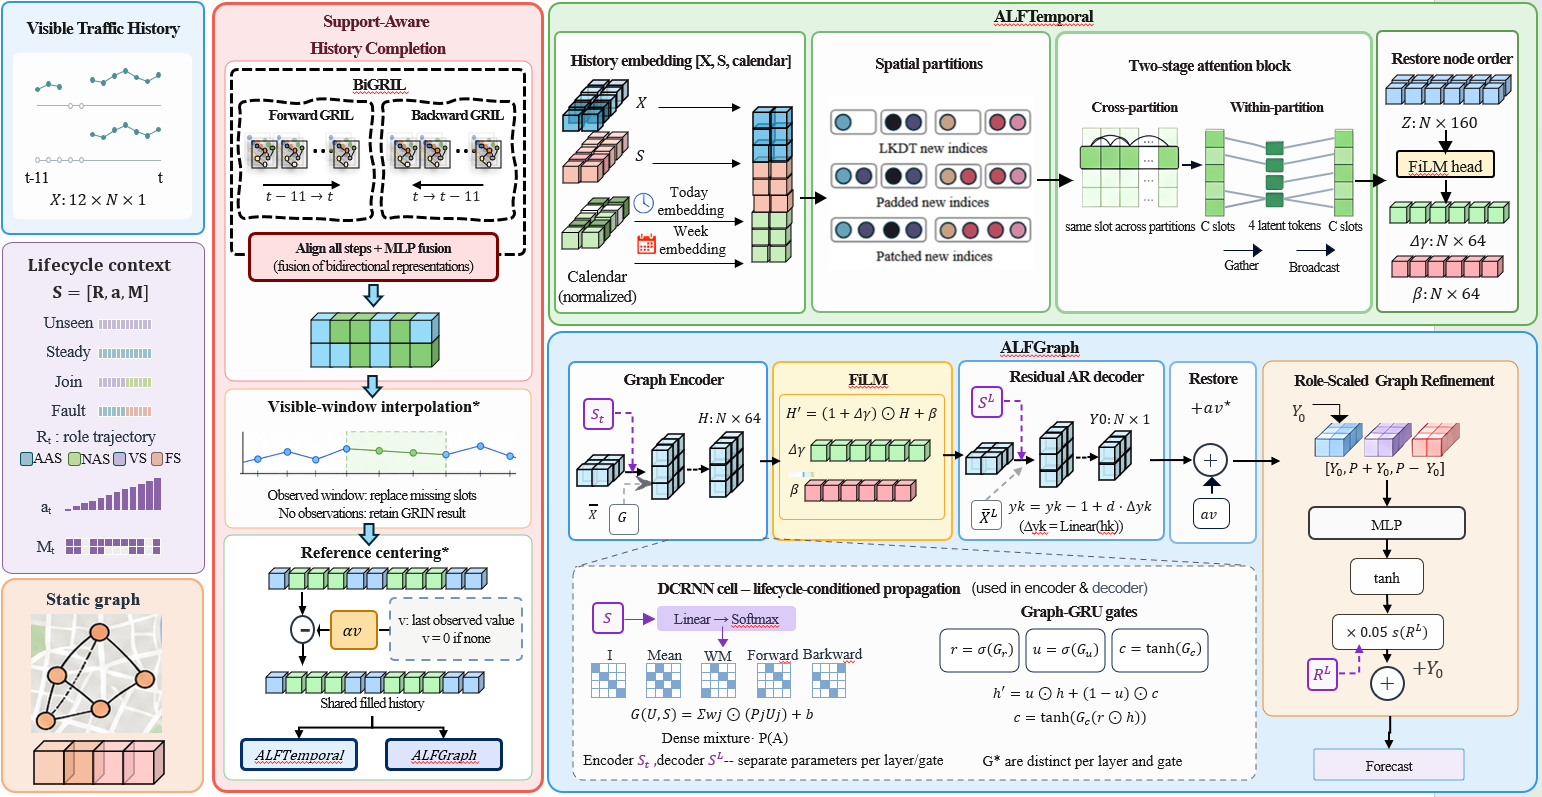
\includegraphics[width=\textwidth]{figures/alfnet.png}
\caption{\textbf{ALFNet 总体架构。}左列为输入：可见历史 $\mathbf{X}$、生命周期上下文 $\mathbf{S}=[\mathbf{R},\mathbf{a},\mathbf{M}]$ 与静态路网（\ref{sec:3_1}节）；第二列为 SAHC（\ref{sec:3_2}节）；右上为 ALFTemporal 及其 FiLM 参数头（\ref{sec:3_3}节）；右下为 ALFGraph，包括 OS 路由的图编码器、FiLM 调制、残差自回归解码、参考恢复与角色缩放图修正（\ref{sec:3_4}节）。}
\label{fig:arch}
\end{figure}

\subsection{问题设置}\label{sec:3_1}

路网表示为有向加权图 $\mathcal{G}=(\mathcal{V},\mathbf{A})$，其中 $|\mathcal{V}|=N$，$\mathbf{A}\in\mathbb{R}_{\ge 0}^{N\times N}$ 为加权邻接矩阵，全部节点的拓扑及静态属性在训练与推理中均可见。节点划分为已知节点 $\mathcal{V}_K$ 以及验证、测试保留节点 $\mathcal{V}_V$、$\mathcal{V}_T$：训练只读取 $\mathcal{V}_K$ 的动态信号，验证与测试分别加入 $\mathcal{V}_V$ 与 $\mathcal{V}_T$ 的历史；标准化统计量仅由训练时段的 $\mathcal{V}_K$ 计算。给定历史长度 $L=12$ 与预测长度 $H=12$，记标准化后的历史为 $\mathbf{X}\in\mathbb{R}^{L\times N}$，未来目标为 $\mathbf{Y}\in\mathbb{R}^{H\times N}$，观测掩码为 $\mathbf{M}\in\{0,1\}^{L\times N}$；$\mathbf{x}_t,\mathbf{m}_t\in\mathbb{R}^{N}$ 为第 $t$ 步全部节点的读数与掩码，即 $\mathbf{X}$ 与 $\mathbf{M}$ 的第 $t$ 行。不可用位置的输入值置零。

\textbf{观测角色与状态进度。} 除掩码外，OS 还由两类逐步的显式描述刻画。在第 $t$ 步，每个节点属于以下四类观测角色之一：AAS 表示节点处于当前阶段的信号暴露范围内，且没有发生接入或失效事件；NAS 表示节点在窗口内接入，接入后开始提供读数；FS 表示节点原本可读，在窗口内失效后不再提供读数；VS 表示节点在该步没有可读历史，包括尚未接入的节点以及不在当前阶段信号暴露范围内的节点（如训练时的保留节点）。$\mathbf{R}_t\in\{0,1\}^{N\times4}$ 依次按 AAS、NAS、VS、FS 对观测角色做 one-hot 编码。状态进度 $\mathbf{a}_t\in[0,1]^{N}$ 描述接入或失效已持续的比例：
\begin{equation}\label{eq:1}
a_{t,n}=\begin{cases}1, & \text{节点 } n \text{ 在第 } t \text{ 步为 AAS},\\ 0, & \text{节点 } n \text{ 在第 } t \text{ 步为 VS},\\ \lambda/L, & \text{节点 } n \text{ 在第 } t \text{ 步为 NAS 或 FS，且处于接入或失效后的第 } \lambda \text{ 步}.\end{cases}
\end{equation}
观测掩码由读数的自然有效性与观测角色共同决定：$M_{t,n}=1$ 当且仅当该读数自然有效且节点在第 $t$ 步为 AAS 或 NAS。自然缺失只改变 $\mathbf{M}$，不改变观测角色，因此 AAS 的偶发缺测仍记为 AAS。三者逐步拼接为生命周期上下文
\begin{equation}\label{eq:2}
\mathbf{S}_t=[\mathbf{R}_t,\ \mathbf{a}_t,\ \mathbf{m}_t]\in\mathbb{R}^{N\times 6},\qquad t=1,\dots,L.
\end{equation}

\textbf{场景。} 按目标节点在窗口内的观测角色轨迹，OS 的变化归纳为四类场景。记 $m\in\{1,\dots,L\}$ 为接入或失效之后已经持续的步数（事件持续步数）：Unseen 中目标节点全程为 VS；Steady 中全程为 AAS；Join 中前 $L-m$ 步为 VS、最后 $m$ 步为 NAS；Fault 中前 $L-m$ 步为 AAS、最后 $m$ 步为 FS。因此，Join 中 $m$ 越大，窗口内可读的新读数越多；Fault 中 $m$ 越大，缺失的近期读数越多。$m$ 在 $1$ 至 $L$ 内均匀抽取；训练时四类场景均在已知节点上模拟。窗口内可见读数数 $q_n=\sum_{t}M_{t,n}$ 只用于描述 OS 的多少，不作为额外输入。本文假设观测角色与状态进度已知，实际应用中可由传感器接入记录与故障检测获得。

\textbf{预测任务。} 在上述设置下，预测是在固定模型参数下学习映射
\begin{equation}\label{eq:3}
\hat{\mathbf{Y}}=f\big(\mathbf{X}\odot\mathbf{M},\ \mathbf{S}_{1:L},\ \mathbf{A},\ \mathcal{T}\big)\in\mathbb{R}^{H\times N},
\end{equation}
其中 $\mathcal{T}$ 为窗口内各步的日历信息（日内时段与星期）。同一节点在不同窗口中可以处于不同观测角色与布局，因此模型应依据当前窗口的 OS 组织计算，而不是依据节点是否参与过训练。

\subsection{观测支持感知历史补全（SAHC）}\label{sec:3_2}

SAHC 对全部 $N$ 个节点、完整的 $L$ 步历史只运行一次，依次进行双向图循环补全、窗口内插值与参考中心化。记 $\mathrm{rn}(\cdot)$ 为矩阵的行归一化（每行除以该行元素之和，全零行保持不变），前向与后向转移矩阵为 $\mathbf{P}_{\mathrm f}=\mathrm{rn}(\mathbf{A})$ 与 $\mathbf{P}_{\mathrm b}=\mathrm{rn}(\mathbf{A}^{\top})$。

\textbf{图门控循环单元。} SAHC 与 ALFGraph 都以图门控循环单元为递推单元。给定输入 $\mathbf{x}$ 与上一隐藏状态 $\mathbf{h}$，单元按
\begin{equation}\label{eq:4}
\begin{aligned}
\mathbf{r}&=\sigma\big(\Phi_r([\mathbf{x},\mathbf{h}])\big),\qquad \mathbf{u}=\sigma\big(\Phi_u([\mathbf{x},\mathbf{h}])\big),\\
\tilde{\mathbf{h}}&=\tanh\big(\Phi_c([\mathbf{x},\mathbf{r}\odot\mathbf{h}])\big),\qquad \mathbf{h}'=\mathbf{u}\odot\mathbf{h}+(\mathbf{1}-\mathbf{u})\odot\tilde{\mathbf{h}}
\end{aligned}
\end{equation}
更新隐藏状态，其中 $\mathbf{r}$、$\mathbf{u}$ 为重置门与更新门，$\tilde{\mathbf{h}}$ 为候选状态，$\sigma(\cdot)$ 为 sigmoid；$\Phi_r$、$\Phi_u$、$\Phi_c$ 为三个参数独立的图变换，输出宽度均为64。SAHC 中三个图变换均取二阶扩散卷积 $\mathcal{D}(\mathbf{U})=[\mathbf{U},\mathbf{P}_{\mathrm f}\mathbf{U},\mathbf{P}_{\mathrm f}^{2}\mathbf{U},\mathbf{P}_{\mathrm b}\mathbf{U},\mathbf{P}_{\mathrm b}^{2}\mathbf{U}]\,\mathbf{W}_{\mathcal{D}}$，记该单元为 $\mathrm{GRU}_{\mathcal{D}}$；ALFGraph 中的图变换在\ref{sec:3_4}节给出。

\textbf{双向图循环补全。} SAHC 沿时间正、反两个方向各运行一个图循环补全层。以正向为例，隐藏状态 $\mathbf{h}_0=\mathbf{0}\in\mathbb{R}^{N\times64}$。对 $t=1,\dots,L$，先由上一隐藏状态给出初步估计，并保留可见位置的观测值：
\begin{equation}\label{eq:5}
\hat{\mathbf{x}}^{(1)}_t=\mathbf{h}_{t-1}\mathbf{W}_1,\qquad \mathbf{x}^{(1)}_t=\mathbf{m}_t\odot\mathbf{x}_t+(\mathbf{1}-\mathbf{m}_t)\odot\hat{\mathbf{x}}^{(1)}_t.
\end{equation}
随后通过一次空间消息传递修正估计：
\begin{equation}\label{eq:6}
\begin{aligned}
\mathbf{z}_t&=[\mathbf{x}^{(1)}_t,\ \mathbf{S}_t,\ \mathbf{h}_{t-1}]\,\mathbf{W}_{\mathrm{in}},\\
\boldsymbol{\rho}_t&=\Big[\mathrm{PReLU}\big(\big[[\mathbf{P}_{\mathrm f}\mathbf{z}_t,\ \mathbf{P}_{\mathrm b}\mathbf{z}_t]\,\mathbf{W}_{\mathrm s},\ \mathbf{h}_{t-1}\big]\,\mathbf{W}_{\mathrm o}\big),\ \mathbf{h}_{t-1}\Big],\qquad \hat{\mathbf{x}}^{(2)}_t=\boldsymbol{\rho}_t\mathbf{W}_2,
\end{aligned}
\end{equation}
其中 $\mathbf{z}_t\in\mathbb{R}^{N\times64}$ 为投影后的输入，$\boldsymbol{\rho}_t\in\mathbb{R}^{N\times128}$ 为该步的节点表示。修正后的估计同样只填入缺失位置，再与生命周期上下文一起更新隐藏状态：
\begin{equation}\label{eq:7}
\mathbf{x}^{(2)}_t=\mathbf{m}_t\odot\mathbf{x}_t+(\mathbf{1}-\mathbf{m}_t)\odot\hat{\mathbf{x}}^{(2)}_t,\qquad \mathbf{h}_t=\mathrm{GRU}_{\mathcal{D}}\big([\mathbf{x}^{(2)}_t,\ \mathbf{S}_t],\ \mathbf{h}_{t-1}\big).
\end{equation}
反向层在时间反转的序列上执行相同计算，参数独立。记正向与反向在第 $t$ 步的节点表示为 $\overrightarrow{\boldsymbol{\rho}}_t$ 与 $\overleftarrow{\boldsymbol{\rho}}_t$，二者在每个历史位置上与掩码拼接，经多层感知机（MLP）融合为重建值，最后保留可见读数：
\begin{equation}\label{eq:8}
\mathbf{x}^{\mathrm{rec}}_t=\mathrm{ReLU}\big([\overrightarrow{\boldsymbol{\rho}}_t,\ \overleftarrow{\boldsymbol{\rho}}_t,\ \mathbf{m}_t]\,\mathbf{W}_3\big)\mathbf{W}_4,\qquad \mathbf{X}^{\mathrm{c}}=\mathbf{M}\odot\mathbf{X}+(\mathbf{1}-\mathbf{M})\odot\mathbf{X}^{\mathrm{rec}},
\end{equation}
其中 $\mathbf{X}^{\mathrm{rec}}=[\mathbf{x}^{\mathrm{rec}}_1,\dots,\mathbf{x}^{\mathrm{rec}}_L]^{\top}$ 为重建结果。式~\eqref{eq:5}–(8)中的 $\mathbf{W}_{\ast}$ 均为可学习矩阵，偏置省略，隐藏宽度与融合 MLP 的宽度均为64。生命周期上下文进入两个方向的每一步递推，掩码还用于保留可见读数与融合。SAHC 没有独立的重建损失，只通过下游预测损失训练。

\textbf{窗口内插值。} 设 $\iota\in\{0,1\}$ 为插值开关。$\iota=1$ 时，对至少有一个可见读数（$q_n>0$）的节点，用窗口内可见读数的线性插值覆盖其缺失位置：
\begin{equation}\label{eq:9}
X^{\mathrm{fill}}_{t,n}=\begin{cases}X_{t^{-},n}+\dfrac{t-t^{-}}{t^{+}-t^{-}}\big(X_{t^{+},n}-X_{t^{-},n}\big), & \iota=1,\ M_{t,n}=0,\ q_n>0,\\[6pt] X^{\mathrm{c}}_{t,n}, & \text{其他情况},\end{cases}
\end{equation}
其中 $t^{-}$ 与 $t^{+}$ 为 $t$ 之前与之后最近的可见步；$t$ 位于第一个可见步之前或最后一个可见步之后时，二者都取最近的可见步并令分式为0，即取最近的可见值。没有可见读数的节点保留 $\mathbf{X}^{\mathrm{c}}$ 中的补全值，因此插值与图循环补全不是按 $q_n$ 互斥的两条支路。

\textbf{参考中心化。} 记 $t^{\ast}_n=\max\{t:M_{t,n}=1\}$ 为节点 $n$ 的最后一个可见步，参考值与中心化后的共享历史为
\begin{equation}\label{eq:10}
v_n=\begin{cases}X_{t^{\ast}_n,n}, & q_n>0,\\ 0, & q_n=0,\end{cases}\qquad \bar{\mathbf{X}}=\mathbf{X}^{\mathrm{fill}}-\alpha\,\mathbf{1}_L\mathbf{v}^{\top},
\end{equation}
其中 $\alpha\ge0$ 为中心化强度，$\mathbf{1}_L$ 为全1列向量，即 $\mathbf{v}$ 沿时间维广播；$\mathbf{S}$ 保持不变。中心化在输出端由式~\eqref{eq:26}加回。上述处理均不使用未来或被遮蔽的真值。保留观测值发生在中心化之前，中心化后可见位置的数值也随之平移。ALFTemporal 与 ALFGraph 读取同一份 $\bar{\mathbf{X}}$。

\subsection{空间上下文时间条件分支（ALFTemporal）}\label{sec:3_3}

ALFTemporal 从跨节点历史生成逐节点的条件特征。它只为 ALFGraph 提供条件，不产生独立预测；计算上先由它得到调制参数，再执行 ALFGraph。

\textbf{时间嵌入。} 对每个节点 $n$，ALFTemporal 读取 $\mathbf{F}_n=[\bar{\mathbf{X}}_{:,n},\ \mathbf{S}_{1:L,n},\ \boldsymbol{\tau}/288,\ \boldsymbol{\delta}/7]\in\mathbb{R}^{L\times9}$，其中 $\bar{\mathbf{X}}_{:,n}$ 为 $\bar{\mathbf{X}}$ 的第 $n$ 列，$\mathbf{S}_{1:L,n}\in\mathbb{R}^{L\times6}$ 为节点 $n$ 在各步的生命周期上下文，$\tau_t=12\cdot\mathrm{hour}_t+\lfloor\mathrm{minute}_t/5\rfloor\in\{0,\dots,287\}$ 为日内时段，$\delta_t\in\{0,\dots,6\}$ 为星期。卷积核长度与步长均为 $L$ 的时间卷积把整个窗口映射为一个64维向量，等价于
\begin{equation}\label{eq:11}
\mathbf{e}_n=\mathrm{vec}(\mathbf{F}_n)\,\mathbf{W}_e+\mathbf{b}_e\in\mathbb{R}^{64},\qquad \mathbf{W}_e\in\mathbb{R}^{9L\times64},
\end{equation}
因此每个节点只有一个时间 patch，窗口内读数的位置信息由 $\mathbf{W}_e$ 的不同行保留。随后拼接日历与结构嵌入：
\begin{equation}\label{eq:12}
\mathbf{z}^{0}_n=\big[\mathbf{e}_n\ \|\ \mathbf{E}^{\mathrm{tod}}_{\tau_L}\ \|\ \mathbf{E}^{\mathrm{dow}}_{\delta_L}\ \|\ \phi(\mathbf{g}_n)\big]\in\mathbb{R}^{160},
\end{equation}
其中 $\|$ 表示拼接，$\mathbf{E}^{\mathrm{tod}}\in\mathbb{R}^{288\times32}$ 与 $\mathbf{E}^{\mathrm{dow}}\in\mathbb{R}^{7\times32}$ 为可学习的日历嵌入表，按末步的日内时段与星期取行。

\textbf{结构嵌入。} 模型不使用逐节点可训练的身份嵌入，以免为保留节点引入可训练的身份参数；结构嵌入由所有节点共享的映射 $\phi$ 作用于静态结构特征 $\mathbf{g}_n\in\mathbb{R}^{7}$ 得到。记 $d^{\mathrm{in}}_n=\sum_{n'\ne n}A_{n'n}$、$d^{\mathrm{out}}_n=\sum_{n'\ne n}A_{nn'}$、$d^{\mathrm{tot}}_n=d^{\mathrm{in}}_n+d^{\mathrm{out}}_n$，$(o^{1}_n,o^{2}_n)$ 为节点的两维坐标（无坐标时置零），则
\begin{equation}\label{eq:13}
\begin{aligned}
\mathbf{g}_n&=\big[\nu(\mathbf{o}^{1})_n,\ \nu(\mathbf{o}^{2})_n,\ \nu(\mathbf{d}^{\mathrm{in}})_n,\ \nu(\mathbf{d}^{\mathrm{out}})_n,\ \nu(\mathbf{d}^{\mathrm{tot}})_n,\ \nu\big(\log(1+\mathbf{d}^{\mathrm{tot}})\big)_n,\ \mathbb{I}[d^{\mathrm{tot}}_n=0]\big],\\
\nu(\mathbf{s})_n&=\frac{s_n-\bar{s}}{\max_{n'}|s_{n'}-\bar{s}|},
\end{aligned}
\end{equation}
其中 $\mathbf{o}^{1}$、$\mathbf{d}^{\mathrm{in}}$ 等表示由全部节点的相应取值组成的向量，$\bar{s}$ 为向量 $\mathbf{s}$ 在全部节点上的均值，$\mathbb{I}[\cdot]$ 为指示函数；$\phi$ 为两层 MLP（$7\to64\to32$，ReLU 激活）。

\textbf{空间分区。} 训练前，节点被划分为 $P=32$ 个分区，每个分区含 $C$ 个槽位：节点坐标可靠时按坐标以 KD-tree 划分，否则依据图拓扑做考虑连通分量的广度优先搜索（BFS）划分。记 $\pi(p,c)$ 为第 $p$ 个分区第 $c$ 个槽位对应的节点；节点不足 $C$ 个的分区以邻接排序的真实节点补足，这些补足副本只提供上下文，不产生输出。按 $\pi$ 排列得到分区张量 $\mathbf{T}\in\mathbb{R}^{P\times C\times160}$，其中 $\mathbf{T}_{p,c}=\mathbf{z}^{0}_{\pi(p,c)}$；下文以 $\mathbf{T}_{:,c}\in\mathbb{R}^{P\times160}$ 表示各分区第 $c$ 个槽位组成的切片，以 $\mathbf{T}_{p,:}\in\mathbb{R}^{C\times160}$ 表示第 $p$ 个分区的全部槽位。

\textbf{两阶段注意力。} 分区张量经一个两阶段注意力块处理。记单头注意力与前馈层为
\begin{equation}\label{eq:14}
\mathrm{Attn}(\mathbf{Q},\mathbf{K},\mathbf{V})=\mathrm{softmax}\Big(\frac{(\mathbf{Q}\mathbf{W}^{Q})(\mathbf{K}\mathbf{W}^{K})^{\top}}{\sqrt{160}}\Big)\mathbf{V}\mathbf{W}^{V}\mathbf{W}^{O},\qquad \mathrm{FFN}(\cdot)=\mathrm{GELU}\big((\cdot)\,\mathbf{W}^{F}_{1}\big)\mathbf{W}^{F}_{2},
\end{equation}
其中各投影矩阵均为 $160\times160$，偏置省略；每次出现的 Attn 与 FFN 各有独立参数。第一阶段为跨分区注意力：对每个槽位 $c$，在 $P$ 个分区的同位 token $\mathbf{T}_{:,c}$ 之间做自注意力，
\begin{equation}\label{eq:15}
\tilde{\mathbf{T}}_{:,c}=\mathrm{LN}\big(\mathbf{T}_{:,c}+\mathrm{Attn}_1(\mathbf{T}_{:,c},\mathbf{T}_{:,c},\mathbf{T}_{:,c})\big),\qquad \mathbf{T}'_{:,c}=\mathrm{LN}\big(\tilde{\mathbf{T}}_{:,c}+\mathrm{FFN}_1(\tilde{\mathbf{T}}_{:,c})\big),
\end{equation}
其中 LN 为层归一化。对 $c=1,\dots,C$ 执行式~\eqref{eq:15}，得到第一阶段输出 $\mathbf{T}'\in\mathbb{R}^{P\times C\times160}$，其中每个 $\mathbf{T}'_{p,c}$ 都已融合其他分区同一槽位的信息。第二阶段在每个分区内部进行：对分区 $p$ 取 $\mathbf{T}'_{p,:}$，由4个可学习的潜在 token $\mathbf{Q}_p\in\mathbb{R}^{4\times160}$ 先从 $C$ 个槽位汇聚信息，再回传给各槽位，
\begin{equation}\label{eq:16}
\begin{aligned}
\mathbf{B}_p&=\mathrm{Attn}_2(\mathbf{Q}_p,\mathbf{T}'_{p,:},\mathbf{T}'_{p,:}),\\
\tilde{\mathbf{T}}_{p,:}&=\mathrm{LN}\big(\mathbf{T}'_{p,:}+\mathrm{Attn}_3(\mathbf{T}'_{p,:},\mathbf{B}_p,\mathbf{B}_p)\big),\qquad \mathbf{T}''_{p,:}=\mathrm{LN}\big(\tilde{\mathbf{T}}_{p,:}+\mathrm{FFN}_2(\tilde{\mathbf{T}}_{p,:})\big).
\end{aligned}
\end{equation}
其中 $\mathbf{B}_p\in\mathbb{R}^{4\times160}$ 为汇聚得到的分区摘要。对 $p=1,\dots,P$ 执行式~\eqref{eq:16}，得到 $\mathbf{T}''\in\mathbb{R}^{P\times C\times160}$。由于第二阶段的输入已经包含跨分区信息，分区内汇聚与回传后，每个槽位同时获得分区内与分区间的上下文；分区内的交互经过4个 token 的瓶颈，而不是 $C\times C$ 的直接注意力。注意力权重与各残差分支上使用 dropout。最后按 $\pi$ 从 $\mathbf{T}''$ 中取回每个真实节点的输出，恢复原始节点顺序，得到条件特征 $\mathbf{Z}\in\mathbb{R}^{N\times160}$，其第 $n$ 行记为 $\mathbf{z}_n$。

\textbf{FiLM 参数头。} FiLM 参数头把 $\mathbf{z}_n$ 映射为逐节点的缩放与平移参数：
\begin{equation}\label{eq:17}
[\Delta\boldsymbol{\gamma}_n,\ \boldsymbol{\beta}_n]=\mathrm{ReLU}\big(\mathbf{z}_n\mathbf{W}_{\gamma,1}+\mathbf{b}_{\gamma,1}\big)\mathbf{W}_{\gamma,2}+\mathbf{b}_{\gamma,2},\qquad \Delta\boldsymbol{\gamma}_n,\ \boldsymbol{\beta}_n\in\mathbb{R}^{64},
\end{equation}
其中 $\mathbf{W}_{\gamma,1}\in\mathbb{R}^{160\times32}$，$\mathbf{W}_{\gamma,2}\in\mathbb{R}^{32\times128}$。最后一层零初始化，训练开始时调制为恒等映射。OS 对调制参数的影响只经由 ALFTemporal 的输入 $\mathbf{S}$，参数头本身不读取 $\mathbf{S}$。

\subsection{观测条件化图预测（ALFGraph）}\label{sec:3_4}

ALFGraph 由 OS 路由的图编码器、FiLM 调制、残差自回归解码器、参考恢复与角色缩放图修正组成，输出唯一的预测 $\hat{\mathbf{Y}}$。

\textbf{OS 路由的图专家混合。} ALFGraph 采用专家混合（mixture of experts，MoE）的思想组织图传播：每个图专家由一个传播算子及其投影组成，路由器依据生命周期上下文为每个节点分配各专家的权重。五个专家的传播算子依次为恒等矩阵 $\mathbf{P}_1=\mathbf{I}$、二值邻接的行归一化 $\mathbf{P}_2=\mathrm{rn}(\mathbb{I}[\mathbf{A}>0])$、加权邻接的行归一化 $\mathbf{P}_3=\mathrm{rn}(\mathbf{A})$，以及前向与后向转移矩阵 $\mathbf{P}_4=\mathbf{P}_{\mathrm f}$、$\mathbf{P}_5=\mathbf{P}_{\mathrm b}$，其中 $\mathbb{I}[\cdot]$ 逐元素取指示函数；第3与第4个专家的传播算子相同，但投影参数与路由权重独立。第 $t$ 步的路由权重只由生命周期上下文决定：
\begin{equation}\label{eq:18}
\mathbf{w}_t=\mathrm{softmax}\big(\mathbf{S}_t\mathbf{W}_g\big)\in\mathbb{R}^{N\times5},
\end{equation}
其中 $\mathbf{W}_g\in\mathbb{R}^{6\times5}$ 为路由矩阵，softmax 对每个节点在5个专家上归一化。给定输入 $\mathbf{U}\in\mathbb{R}^{N\times F}$，图专家混合的输出为
\begin{equation}\label{eq:19}
G(\mathbf{U},\mathbf{S}_t)=\sum_{j=1}^{5}\mathbf{w}_{t,j}\odot\big(\mathbf{P}_j\,\mathbf{U}\,\boldsymbol{\Theta}_j\big)+\mathbf{b},
\end{equation}
其中 $\mathbf{w}_{t,j}\in\mathbb{R}^{N}$ 为 $\mathbf{w}_t$ 的第 $j$ 列，即各节点分配给第 $j$ 个专家的权重，沿特征维广播；$\boldsymbol{\Theta}_j\in\mathbb{R}^{F\times64}$ 为第 $j$ 个专家的投影，$\mathbf{b}\in\mathbb{R}^{64}$ 为偏置。五个专家全部参与加权，不做 top-$k$ 截断，也不加入噪声。路由器读取 OS 而非信号值：经过 SAHC 后，一个 NAS 节点与一个 AAS 节点可能具有相似的输入数值，而二者的生命周期上下文仍然不同。

为避免路由集中到少数专家，每次调用图专家混合时计算负载平衡损失。记该次调用中批次内全部样本、全部节点的路由权重为 $w_{n,j}$（$n$ 遍历这些节点，$j=1,\dots,5$），则
\begin{equation}\label{eq:20}
\mathrm{imp}_j=\sum_{n}w_{n,j},\qquad \mathrm{load}_j=\sum_{n}\mathbb{I}[w_{n,j}>0],\qquad \ell_{\mathrm{bal}}=0.01\big[\mathrm{CV}^2(\mathbf{imp})+\mathrm{CV}^2(\mathbf{load})\big],
\end{equation}
其中 $\mathbf{imp}=(\mathrm{imp}_1,\dots,\mathrm{imp}_5)$ 与 $\mathbf{load}$ 分别为各专家获得的权重总和与被分配的节点数，$\mathrm{CV}^2(\cdot)$ 为平方变异系数，即向量各分量的方差除以均值的平方（分母加 $10^{-10}$）。ALFGraph 共有12个图专家混合模块（编码器与解码器各两层，每层三个门）。记 $\mathcal{C}_g$ 为第 $g$ 个模块在一次前向计算中各次调用的平衡损失组成的集合，路由平衡损失为
\begin{equation}\label{eq:21}
\mathcal{L}_{\mathrm{route}}=\frac{1}{12}\sum_{g=1}^{12}\frac{1}{|\mathcal{C}_g|}\sum_{\ell_{\mathrm{bal}}\in\mathcal{C}_g}\ell_{\mathrm{bal}}.
\end{equation}
由于五个专家全部参与加权，$\mathbf{load}$ 的各分量相同，$\mathrm{CV}^2(\mathbf{load})=0$，起作用的是 importance 项。

\textbf{图编码器。} ALFGraph 的图门控循环单元沿用式~\eqref{eq:4}的门控形式，三个图变换 $\Phi_r$、$\Phi_u$、$\Phi_c$ 分别取为各带路由器的图专家混合 $G_r(\cdot,\mathbf{S})$、$G_u(\cdot,\mathbf{S})$、$G_c(\cdot,\mathbf{S})$，隐藏宽度为64，记为 $\mathbf{h}'=\mathrm{Cell}(\mathbf{x},\mathbf{h},\mathbf{S})$。各模块参数在递推步之间共享。编码器从零状态出发，对 $t=1,\dots,L$ 递推
\begin{equation}\label{eq:22}
\mathbf{h}^{(1)}_t=\mathrm{Cell}^{(1)}_{\mathrm{enc}}\big([\bar{\mathbf{x}}_t,\mathbf{S}_t],\ \mathbf{h}^{(1)}_{t-1},\ \mathbf{S}_t\big),\qquad \mathbf{h}^{(2)}_t=\mathrm{Cell}^{(2)}_{\mathrm{enc}}\big(\mathbf{h}^{(1)}_t,\ \mathbf{h}^{(2)}_{t-1},\ \mathbf{S}_t\big),
\end{equation}
其中 $\bar{\mathbf{x}}_t$ 为 $\bar{\mathbf{X}}$ 的第 $t$ 行，第一层输入 $[\bar{\mathbf{x}}_t,\mathbf{S}_t]\in\mathbb{R}^{N\times7}$，$\mathbf{h}^{(l)}_t$ 为第 $l$ 层在第 $t$ 步的隐藏状态。由于观测角色与状态进度逐步进入路由，Join 节点在接入前后、Fault 节点在失效前后会使用不同的专家组合。

\textbf{FiLM 调制。} 编码完成后，ALFTemporal 给出的参数在解码开始前一次性调制两层编码末状态：
\begin{equation}\label{eq:23}
\mathbf{h}^{(l)}_{\mathrm{mod}}=(\mathbf{1}+\Delta\boldsymbol{\gamma})\odot\mathbf{h}^{(l)}_L+\boldsymbol{\beta},\qquad l=1,2,
\end{equation}
其中 $\Delta\boldsymbol{\gamma},\boldsymbol{\beta}\in\mathbb{R}^{N\times64}$ 由式~\eqref{eq:17}逐节点堆叠得到。同一组参数广播到两层，不在每个预测步重新生成。

\textbf{残差自回归解码。} 解码器以调制后的状态为初始隐藏状态，记 $\mathbf{h}^{(l)}_{L}\leftarrow\mathbf{h}^{(l)}_{\mathrm{mod}}$，并以 $\mathbf{y}_0=\bar{\mathbf{x}}_L$ 为初值；该初值来自补全与中心化后的历史，不一定是最后一次真实观测。对 $k=1,\dots,H$，
\begin{equation}\label{eq:24}
\begin{aligned}
\mathbf{h}^{(1)}_{L+k}&=\mathrm{Cell}^{(1)}_{\mathrm{dec}}\big(\mathbf{y}^{\mathrm{in}}_{k-1},\ \mathbf{h}^{(1)}_{L+k-1},\ \mathbf{S}_L\big),\qquad \mathbf{h}^{(2)}_{L+k}=\mathrm{Cell}^{(2)}_{\mathrm{dec}}\big(\mathbf{h}^{(1)}_{L+k},\ \mathbf{h}^{(2)}_{L+k-1},\ \mathbf{S}_L\big),\\
\mathbf{y}_k&=\mathbf{y}^{\mathrm{in}}_{k-1}+d\cdot\big(\mathbf{h}^{(2)}_{L+k}\mathbf{W}_y+b_y\big),
\end{aligned}
\end{equation}
其中 $\mathbf{y}^{\mathrm{in}}_{k-1}$ 为第 $k$ 步的解码输入，$\mathbf{y}^{\mathrm{in}}_0=\mathbf{y}_0$；$\mathbf{W}_y\in\mathbb{R}^{64\times1}$ 与 $b_y$ 为输出投影，$d$ 为解码残差倍率；$\mathbf{h}^{(l)}_{L+k}$ 表示解码第 $k$ 步第 $l$ 层的隐藏状态，解码单元与编码单元参数独立。解码阶段没有未来的生命周期上下文，路由统一使用末步上下文 $\mathbf{S}_L$，不对未来观测角色的演变建模。下一步的输入 $\mathbf{y}^{\mathrm{in}}_k$ 在推理时等于未经修正的 $\mathbf{y}_k$；训练时采用受合法目标掩码约束的 Teacher Forcing：
\begin{equation}\label{eq:25}
\mathbf{y}^{\mathrm{in}}_k=\boldsymbol{\kappa}_k\odot\big(\mathbf{y}^{\ast}_k-\alpha\mathbf{v}\big)+(\mathbf{1}-\boldsymbol{\kappa}_k)\odot\mathbf{y}_k,\qquad \boldsymbol{\kappa}_k=\xi_k\,\boldsymbol{\mu}_k,\qquad \xi_k\sim\mathrm{Bernoulli}\big(\max(0,\,1-i/40)\big),
\end{equation}
其中 $\mathbf{y}^{\ast}_k$ 为 $\mathbf{Y}$ 的第 $k$ 行，减去 $\alpha\mathbf{v}$ 使其与解码器处于同一中心化尺度；$\boldsymbol{\mu}_k\in\{0,1\}^{N}$ 标记第 $k$ 步可合法读取的目标；$i$ 为训练轮次，每个样本的每个预测步独立抽取 $\xi_k$。因此 Teacher Forcing 的比例在前40轮线性衰减至零，推理时 $\boldsymbol{\kappa}_k=\mathbf{0}$。

\textbf{参考恢复。} 完成 $H$ 步解码后加回中心化参考值：
\begin{equation}\label{eq:26}
\tilde{\mathbf{Y}}=[\mathbf{y}_1,\dots,\mathbf{y}_H]^{\top}+\alpha\,\mathbf{1}_H\mathbf{v}^{\top}.
\end{equation}
这一步只恢复式~\eqref{eq:10}减去的参考值，不是标准化的逆变换；误差计算时再用训练时段的标准化统计量还原到原始单位。

\textbf{角色缩放图修正。} 输出端施加一个有界的邻域修正。令 $\mathbf{P}^{+}=\mathrm{rn}(\mathbf{A}+\mathbf{I})$、$\mathbf{P}^{-}=\mathrm{rn}\big((\mathbf{A}+\mathbf{I})^{\top}\big)$，$\tilde{\mathbf{y}}_k$ 为 $\tilde{\mathbf{Y}}$ 的第 $k$ 行，对每个预测步，
\begin{equation}\label{eq:27}
\mathbf{D}_k=\mathrm{GELU}\big([\tilde{\mathbf{y}}_k,\ \mathbf{P}^{+}\tilde{\mathbf{y}}_k,\ \mathbf{P}^{-}\tilde{\mathbf{y}}_k]\,\mathbf{W}_{r,1}+\mathbf{b}_{r,1}\big)\mathbf{W}_{r,2}+\mathbf{b}_{r,2},\qquad \hat{\mathbf{y}}_k=\tilde{\mathbf{y}}_k+0.05\cdot s(\mathbf{R}_L)\odot\tanh(\mathbf{D}_k),
\end{equation}
其中拼接沿每个节点的特征维进行，$\mathbf{W}_{r,1}\in\mathbb{R}^{3\times32}$，$\mathbf{W}_{r,2}\in\mathbb{R}^{32\times1}$ 与 $\mathbf{b}_{r,2}$ 零初始化；$s(\mathbf{R}_L)=\mathbf{R}_L\boldsymbol{\varsigma}$ 按末步观测角色取固定倍率，$\boldsymbol{\varsigma}=(0,1,1,0.25)^{\top}$ 依次对应 AAS、NAS、VS、FS。最终预测为 $\hat{\mathbf{Y}}=[\hat{\mathbf{y}}_1,\dots,\hat{\mathbf{y}}_H]^{\top}$。由于 tanh 有界，修正量的绝对值在标准化单位下不超过0.05。末步为 AAS 的节点自身不被修正，但仍作为邻居参与其他节点的修正。该模块只读取末步观测角色，不读取状态进度与掩码，也没有独立的路由器；修正结果不回送解码器。

\subsection{训练目标}\label{sec:3_5}

令 $\hat{y}$ 与 $y$ 为原始单位下的预测值与真实值，$e=|\hat{y}-y|$ 为绝对误差，$\sigma_{\mathrm{data}}$ 为训练时段目标变量的标准差。逐元素损失为
\begin{equation}\label{eq:28}
\ell(e)=\frac{e}{\sigma_{\mathrm{data}}}\tanh(0.1\,e).
\end{equation}
该损失在小误差附近近似 $0.1e^2/\sigma_{\mathrm{data}}$，大误差时趋近标准化 MAE；权重项参与梯度计算。记 $\Omega$ 为一个批次内真值可用的目标元素，$\Omega_r$ 为其中末步观测角色为 $r$ 的节点所对应的元素，$\mathcal{R}_b$ 为该批次实际出现的观测角色集合，则
\begin{equation}\label{eq:29}
\mathcal{L}_{\mathrm{mean}}=\frac{1}{|\Omega|}\sum_{\Omega}\ell(e),\qquad
\mathcal{L}_{\mathrm{role}}=\frac{1}{|\mathcal{R}_b|}\sum_{r\in\mathcal{R}_b}\frac{1}{|\Omega_r|}\sum_{\Omega_r}\ell(e),
\end{equation}
其中 $\mathcal{L}_{\mathrm{mean}}$ 为全部目标元素上的平均损失；$\mathcal{L}_{\mathrm{role}}$ 先在每个观测角色内部平均，再对批次中出现的角色取平均，使样本较少的角色在优化中获得与其他角色相同的权重。总训练目标为
\begin{equation}\label{eq:30}
\mathcal{L}=0.9\,\mathcal{L}_{\mathrm{mean}}+0.1\,\mathcal{L}_{\mathrm{role}}+\mathcal{L}_{\mathrm{route}},
\end{equation}
其中 $\mathcal{L}_{\mathrm{route}}$ 为式~\eqref{eq:21}的路由平衡损失。训练目标不含独立的重建损失或额外预测头。
